\documentclass[letterpaper, 11pt]{article}
%\usepackage[hmargin = 1in, vmargin = 1in]{geometry}
\usepackage{amsmath}
\usepackage{amssymb}
\usepackage{enumitem}
\usepackage{mathrsfs}
\usepackage{tikz}
\usepackage{graphicx}
\usepackage{algorithmicx}
\usepackage{algpseudocode}
\usepackage{syntax}
\usepackage{adjustbox}
\setlength{\headheight}{14pt}
\usepackage{fancyhdr}
\pagestyle{fancy}
\rhead{Gabriel Wallace}
\lhead{Comp Sci 4250}

\newcommand{\card}{\text{Card}}
\newcommand{\N}{\mathbb{N}}
\newcommand{\R}{\mathbb{R}}
\newcommand{\Z}{\mathbb{Z}}
\newcommand{\Q}{\mathbb{Q}}

\newcommand{\inv}{^{-1}}
\newcommand{\abs}[1]{\lvert #1 \rvert}
\newcommand{\hwnumber}[1]{\medskip \noindent\textbf{#1.} \smallskip}
\newcommand{\hwnumbersec}[3]{\medskip \noindent\textbf{#1.} Chapter #2 \##3 \smallskip}
\newcommand{\A}{\noindent\textbf{A:} }
\newcommand{\Mod}[1]{\ \mathrm{mod}\ #1}
\newcommand{\Alg}[1]{\medskip \noindent\textbf{ALGORITHM} \( #1 \)} 
\newcommand{\To}{$\rightarrow$ }

\newcommand{\tabitem}{~~\llap{\textbullet}~~}

\begin{document}
\begin{center}
	{\LARGE Homework 3}\\
\end{center}

\hwnumber{1}

\begin{center}
\begin{adjustbox}{width={\textwidth},keepaspectratio}
\begin{tabular}{c | l l}
	& Static & Stack dynamic \\
	\hline
	Advantages & \tabitem Quick to allocate/deallocate & \tabitem Support for recursion\\
		   & \tabitem Subprograms can be history sensitive & \tabitem Storage is shared among some subprograms\\
	Disadvantages & \tabitem Does not support recursion & \tabitem Takes longer to allocate/deallocate \\
		      & \tabitem Subprograms cannot share storage & \tabitem Subprograms cannot be history sensitive \\
\end{tabular}
\end{adjustbox}
\end{center}

\hwnumber{2}

When calling subprograms as parameters and the language in use allows nested
subprograms, it is ambiguous as to which referencing environment is used to
execute the passed subprogram. One approach is \textbf{shallow binding} where
the environment of the call statement that executes the passed subprogram is
used. Another approach is \textbf{deep binding} where the environment of the
definition of the passed subprogram is used. 

\hwnumbersec{3}{9}{5}

\begin{enumerate}[label=(\textbf{\alph*})]
	\item Pass by value doesn't change the value of the arguments outside of
		the function definition so the values of \texttt{value} and
		\texttt{list} remain unchanged.
	\item 
		\begin{tabular}{c c}
			\texttt{value} & \texttt{list} \\
			\hline
			1 & \{2, 3, 5, 7, 9\}\\
			1 & \{3, 2, 5, 7, 9\}\\
			2 & \{3, 1, 5, 7, 9\}
	\end{tabular}
\end{enumerate}

\hwnumbersec{4}{9}{7}

\begin{enumerate}[label=(\textbf{\alph*})]
	\item Pass by value doesn't change the value of the arguments outside of
		the function definition so the values of  \texttt{list} remain
		unchanged.
	\item 
		\texttt{list = \{2, 6\}}
\end{enumerate}

\newpage
\hwnumbersec{5}{10}{3}

ARI (see figure \ref{fig:ari}):

\begin{figure}[h]
	\centering
	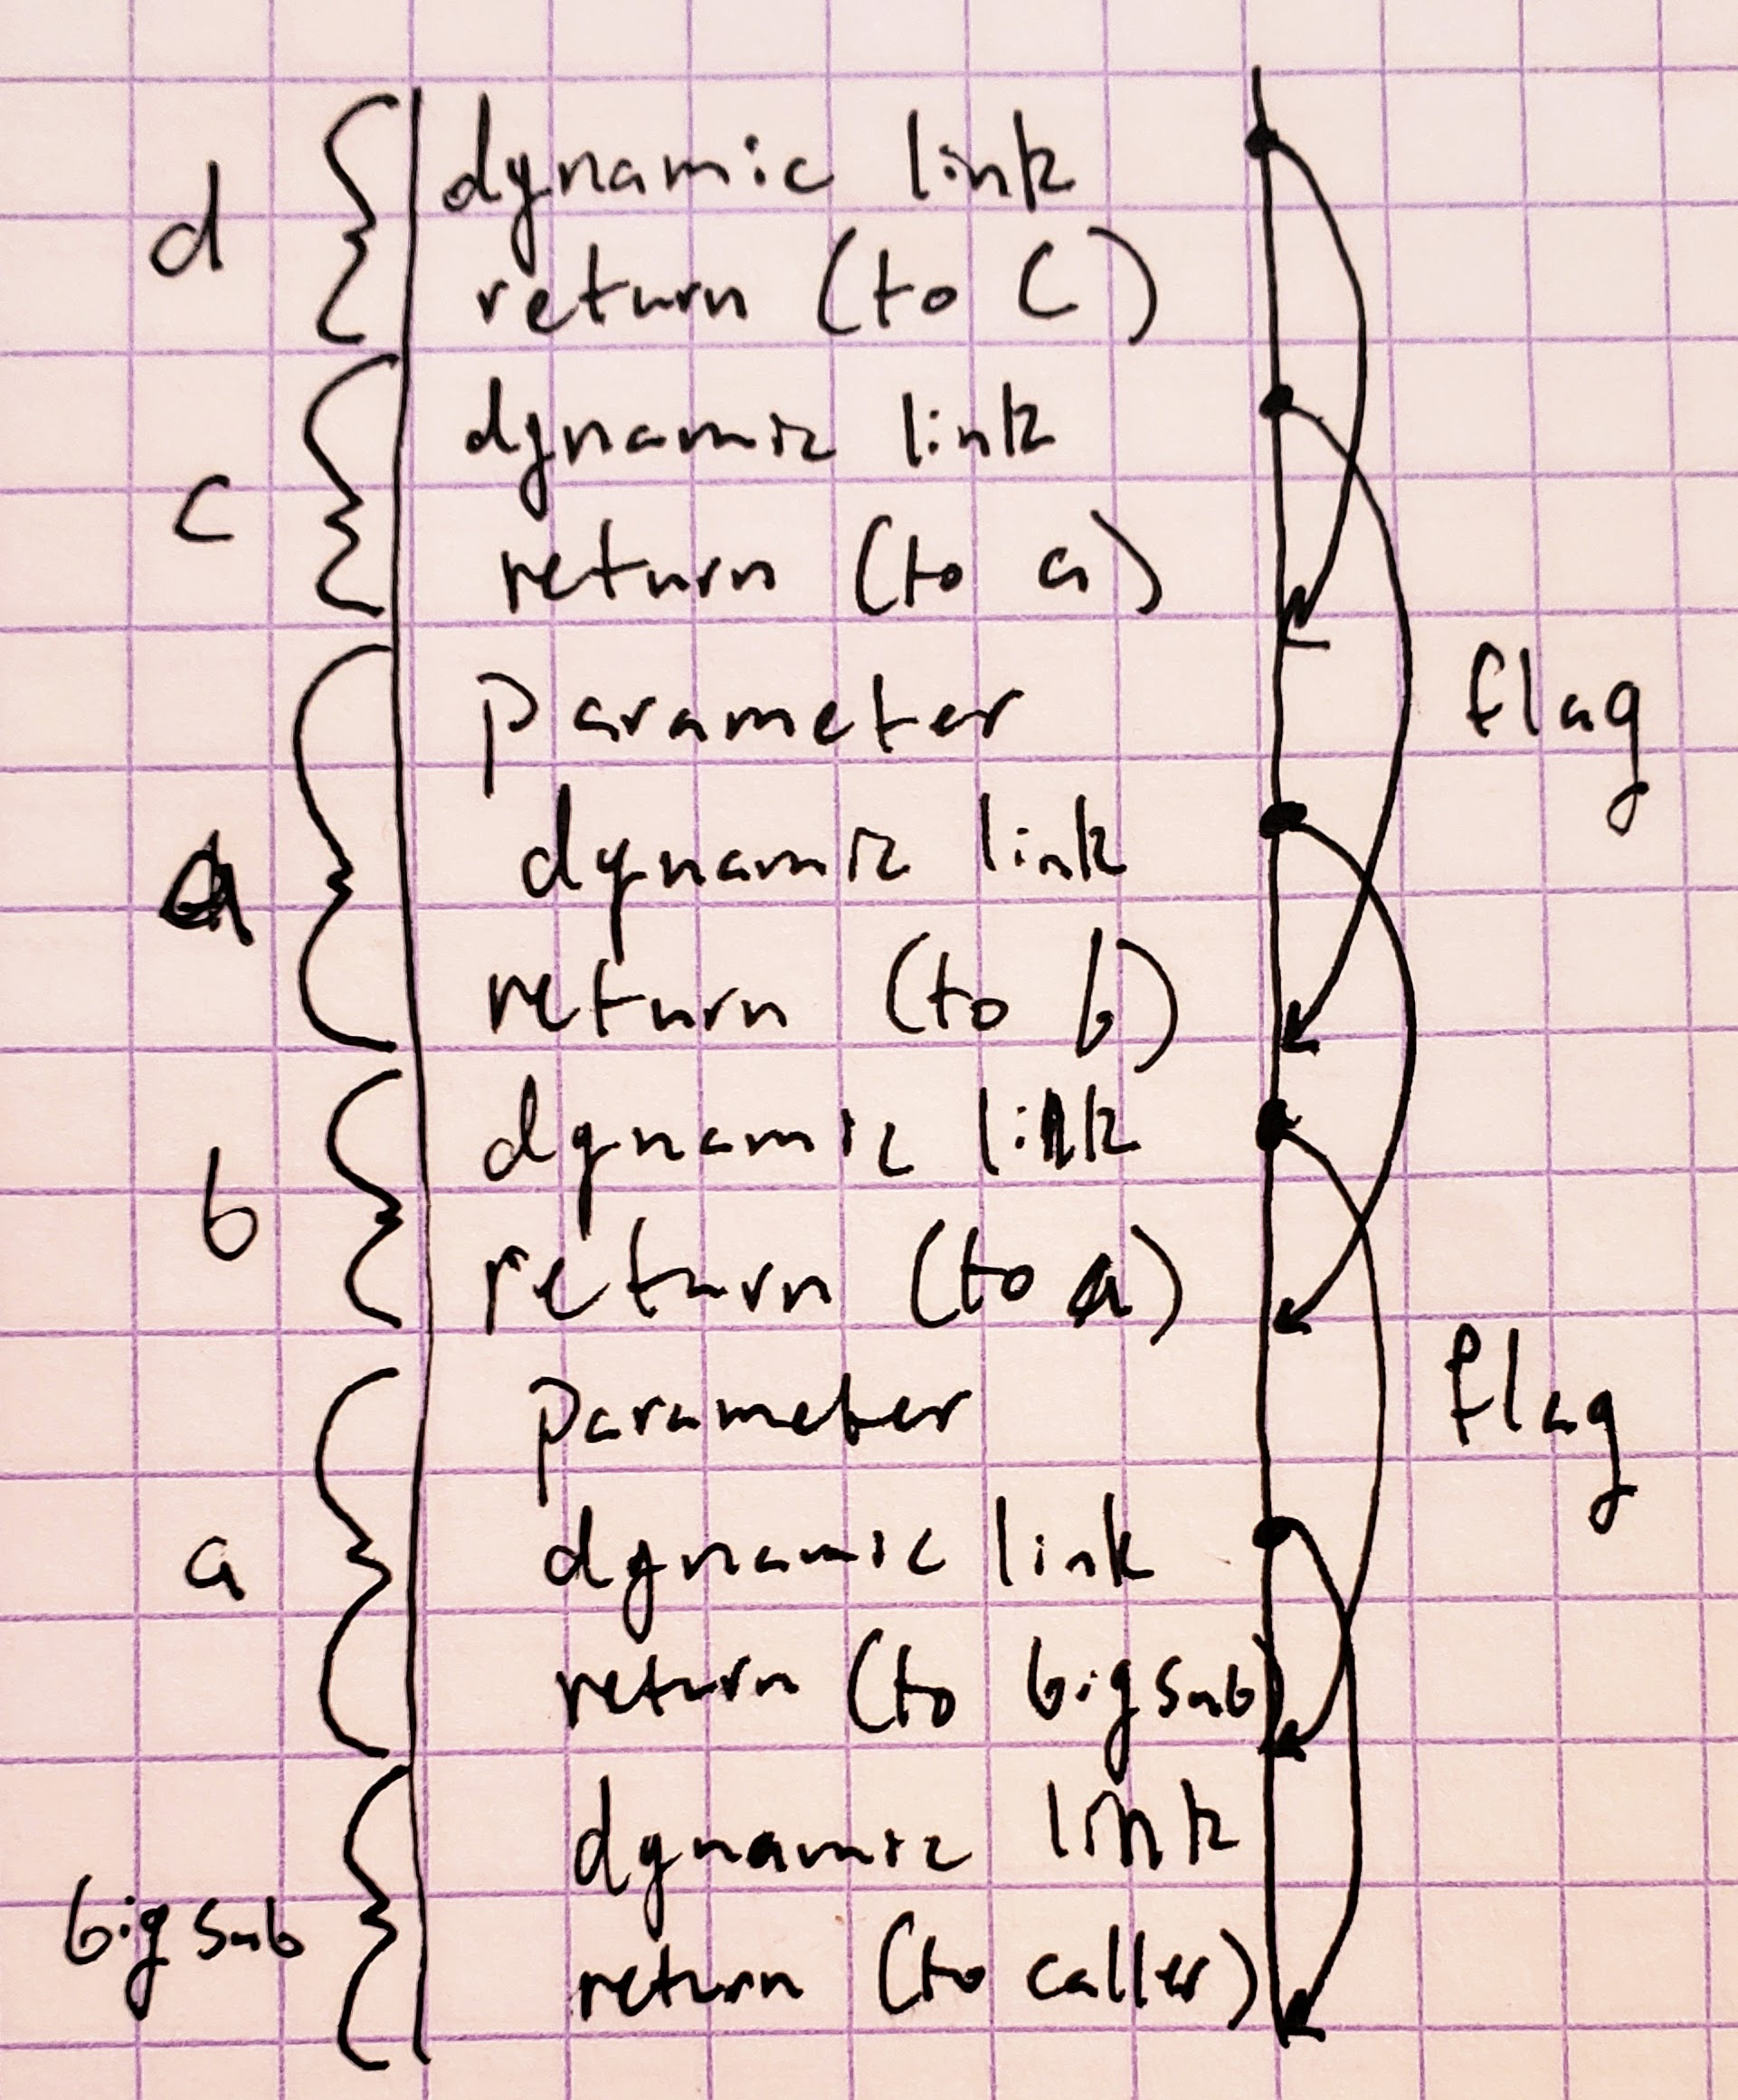
\includegraphics[scale = 0.1]{hw03q5.jpg}
	\caption{ARI for question 5}
	\label{fig:ari}
\end{figure}

\end{document}
